\chapter{Conclusion}\label{ch:conclusion}
\noindent This chapter outlines future research heading and discuss quality of MPC control used with movement automaton $\mathscr{MA}$ control.

\section{Summary of simulation}
\noindent Simulation of system $\dot{x}=f(x,\mathscr{MA})$ show that MPC controller is feasible for plant (\ref{eq:simple3ddifferentialequations}) control.  
\begin{figure}[H]
    \centering
    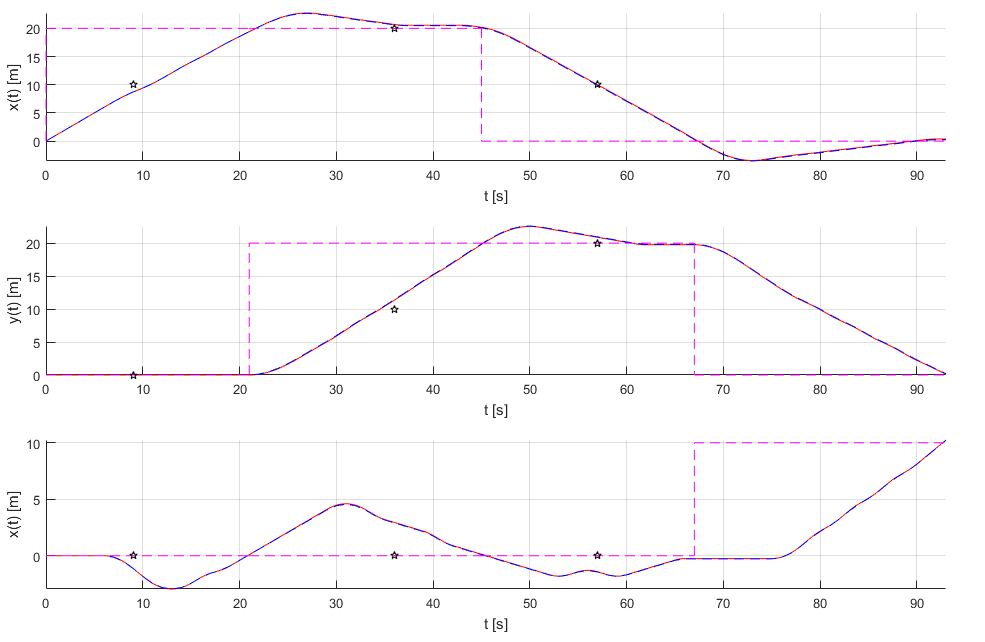
\includegraphics[width=\linewidth]{\FIGDIR/74_MPC_Performance.png}
    \caption{MPC performance at trajectory tracking $[x(t),y(t),z(t)]$.}
    \label{fig:mpcPerformance}
\end{figure}
\noindent Predictor defined by (\ref{eq:discretePredictionChaining}) predicts future parameters $\hat{x}(t)$ with great precision as summarized in figures \ref{fig:vehicleStateKnown1}. and \ref{fig:vehicleStateKnown2}. For playground defined in section \ref{ch:3DPlaygroundDefinition} the mission was executed successfully fig. \ref{fig:55fourthObstacleknown}. Prediction error $e_p$ (\ref{eq:movementAutomatonPredictionError}) was near zero for for all parameters in model (\ref{eq:simple3ddifferentialequations}). Overall performance of approach is more than good. The stability and convertibility of controll approach has been proven in sections \ref{s:maConvergence} and \ref{s:maLyapunov}. Now take look into MPC control quality and summarize control tracking. Figure \ref{fig:mpcPerformance} shows MPC tracking of mission plan given by waypoint set $\mathscr{WP}$ in terms of $x(t)$, $y(t)$ and $z(t)$ with following legend:
\begin{enumerate}
    \item \textit{Reference trajectory} - denoted as dashed magenta line, reference trajectory was generated as straight line segments between waypoints $\mathscr{WP}_S,\dots,\mathscr{WP}_E$. The real system with constrained dynamics can not follow this trajectory, because transition dynamics saturation is achieved over time.  
    \item \textit{Predicted output} - denoted as dashed blue line. Predicted trajectory was following reference trajectory best to its extent. Only deviations from reference trajectory can be seen in $z(t)$ parameter because of the obstacle avoidance. Vehicle was using upward and downward avoidance in case of these trajectories.
    \item \textit{Measured (real) output} - denoted as solid red line. Real system output follows the predicted system state, small unnoticeable deviations were detected due to non-linearity of original vehicle plant. The deviations at movement execution $m_i(t_i)$ time $t_i$ were close to numeric rounding error of environment.
    \item \textit{Obstacle center mass} - denoted as black pentagrams are center of masses for obstacle subsets $\mathscr{O}_1$, $\mathscr{O}_2$ and $\mathscr{O}_3$. They are plotted at avoidance time $t_a$, when obstacle body was tangent to system trajectory.
\end{enumerate}

\section{Future research}
\noindent The future research will use results of this work especially linearized predictor for vehicle plant for fast numeric reach set estimation in sensory FOV of vehicle. Trajectory predictor can predict multiple trajectories in partially constrained FOV, for different goals. These goals can be set as specific parts of visible space in FOV.
